%\documentclass[tikz,convert={outfile=\jobname.svg}]{standalone}
\documentclass[12pt,landscape]{article}

\usepackage[T1]{fontenc}
\usepackage{lmodern}
\usepackage{amsmath}
\usepackage{amssymb}
\usepackage{bm}
\usepackage{tikz}

\usetikzlibrary{arrows,backgrounds,calc,decorations.pathmorphing,fit,matrix,positioning}

\definecolor{dark1}{HTML}{E41A1C}
\definecolor{dark2}{HTML}{377Eb8}
\definecolor{dark3}{HTML}{4DAF4A}
\definecolor{dark4}{HTML}{984EA3}
\definecolor{A1}{HTML}{1b9e77}
\definecolor{A2}{HTML}{d95f02}

\definecolor{R1}{HTML}{fee0d2}
\definecolor{R2}{HTML}{fc9272}
\definecolor{R3}{HTML}{de2d26}

\DeclareMathOperator*{\argmax}{\arg\!\max}
\def\layersep{2.1cm}
\pagestyle{empty}
\begin{document}
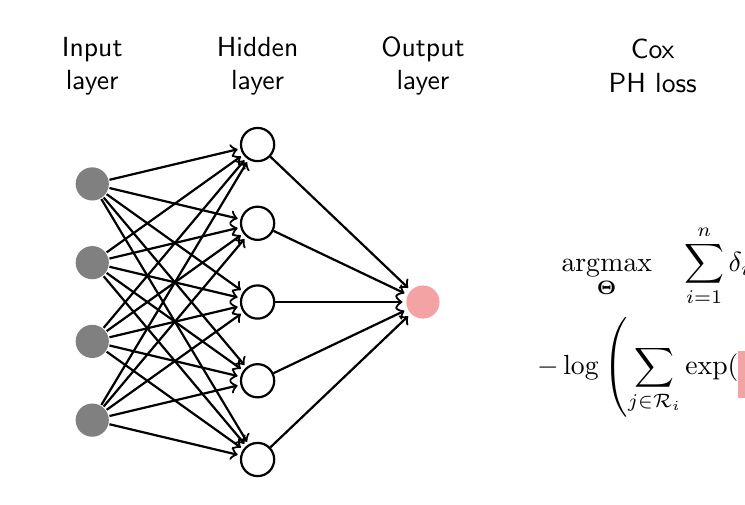
\begin{tikzpicture}[remember picture,thick,shorten >=1pt,->,draw=black, node distance=\layersep]
\tikzstyle{every pin edge}=[<-,shorten <=1pt]
\tikzstyle{neuron}=[circle,minimum size=12pt,inner sep=0pt]
\tikzstyle{input neuron}=[neuron, fill=black!50];
\tikzstyle{output neuron}=[neuron, fill=dark1!40];
\tikzstyle{hidden neuron}=[neuron,draw=black];
\tikzstyle{annot} = [text width=4em, text centered,font=\sffamily]

% Draw the input layer nodes
\foreach \name / \y in {1,...,4}
% This is the same as writing \foreach \name / \y in {1/1,2/2,3/3,4/4}
\node[input neuron] (I-\name) at (0,-\y) {};

% Draw the hidden layer nodes
\foreach \name / \y in {1,...,5}
\path[yshift=0.5cm]
node[hidden neuron] (H-\name) at (\layersep,-\y cm) {};

% Draw the output layer node
\node[output neuron,right of=H-3] (O) {};

% Connect every node in the input layer with every node in the
% hidden layer.
\foreach \source in {1,...,4}
\foreach \dest in {1,...,5}
\path (I-\source) edge (H-\dest);

% Connect every node in the hidden layer with the output layer
\foreach \source in {1,...,5}
\path (H-\source) edge (O);

% Annotate the layers
\node[annot,above of=H-1, node distance=1cm] (hl) {Hidden layer};
\node[annot,left of=hl] {Input layer};
\node[annot,right of=hl] (ol) {Output layer};
\node[annot,right=1.25cm of ol] {Cox PH loss};

%%%
%% RIGHT
%%%
\node[right=1cm of O,text width=1.5cm] {%
\begin{multline*}
\argmax_{\bm{\Theta}}\quad \sum_{i=1}^n \delta_i \left[
\tikz[baseline,remember picture] { \draw node[fill=dark1!40] (m1) {$o(\mathbf{x}_i\,|\,\bm{\Theta})$}; } \right. \\
\left.
- \log \left( \sum_{j \in \mathcal{R}_i} \exp(
\tikz[baseline,remember picture] { \draw node[fill=dark1!40] (m2) {$o(\mathbf{x}_j\,|\,\bm{\Theta})$}; })
\right) \right]\end{multline*}};
\end{tikzpicture}%

\begin{tikzpicture}[overlay,remember picture,-latex,thick,dark1]
%\path (O) edge[bend left,in=135,relative] (m1.north);
\draw (O) .. controls +(1cm,2cm) and +(-1cm,2cm) .. (m1.north);
\path (O) edge[bend right,in=225,relative] (m2.south);
\end{tikzpicture}%
\end{document}